\documentclass[12pt]{article}
\usepackage{fullpage}
\usepackage{multicol}
\usepackage{graphicx}
\usepackage{fontspec}
\usepackage{amsfonts}
\usepackage{mathrsfs}
\usepackage{graphicx}
\usepackage{setspace}
\doublespacing
\setmainfont{OpenDyslexicAlta}
\newcommand{\blk}{\underline{\hspace{0.5in}}}
\begin{document}
%\maketitle
\center{\section*{Geometry Test 1 Spring 2020}}
\center{\section*{Work in your notebook.  Show all work for credit!}}
%\begin{multicols}{2}
\begin{enumerate}

\item You have a 60\% solution of acid, and 5\% solution of acid.  How much of each should
you mix together to make 10 liters of 20\% solution?

\item For each statement, tell me if it is true or false.  If it is false, give a counterexample.
\begin{enumerate}
	\item If you have 2 quarters then you have 50 cents.
	\item If you have 50 cents then you have 2 quarters.
	%\item If a four sided polygon has all lengths equal, then it is a square.
	\item If a polygon is a square, then it has four equal sides.
	%\item A four sided polygon is a square iff that polygon has all equal sides.  
\end{enumerate}

\item Perform the following steps:
\begin{enumerate}
	\item Draw a line $\mathscr{L}$ and a point $p$ not on that line in your notebook.
	\item Draw the line perpendicular to $\mathscr{L}$ through the point $p$ using the construction you have learned.
\end{enumerate}

\item Solve the following equation for $y$:
$$2y + 8x + 4 = 8$$


\item Give an example of a convex polygon.

\item Give an example of a polygon that is \textbf{not} convex.

\item In the picture below $ABCD$ is a rhombus, a polygon with all sides equal.  Prove that the diagonals $\overline{AC}$ and $\overline{BD}$ are perpendicular bisectors of each other.

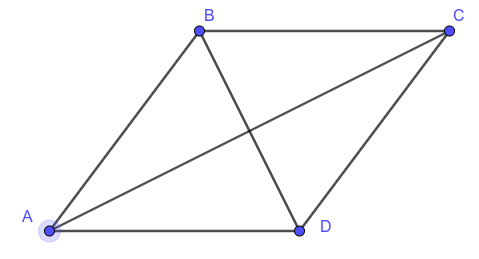
\includegraphics[width=3in]{geom-test3-img2.png}

\item In the diagram below $\triangle ABC$ is an isosceles triangle with $|AC| = |BC|$.
If $m \angle A = 40^o$, what are the measures of the other angles?

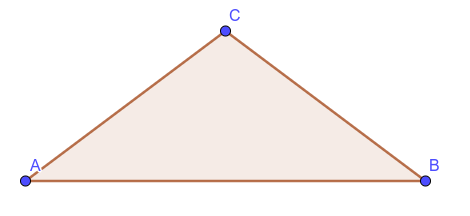
\includegraphics[width=3in]{geom-test3-img1.png}

\newpage

\item In the diagram below $\overline{AB}$ is a diameter through the center $P$ of the circle:

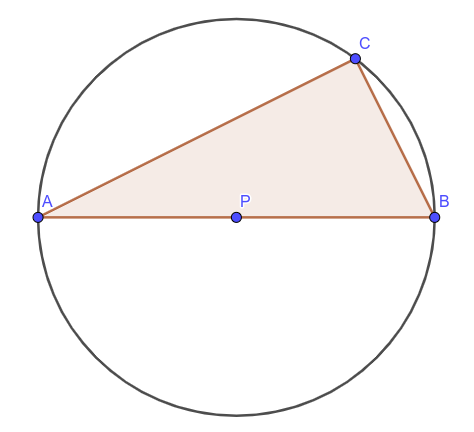
\includegraphics[width=4in]{geom-test3-img3.png}

\begin{enumerate}
	\item What is the measure of the angle $\angle C$?
	\item If the arc $\stackrel \frown {BC}$ has measure $48^o$, what are the other angles of the triangle $\triangle ABC$?
\end{enumerate}


\item How many sides does a polygon have if the sum of its angles is $1440^o$.

\item Inscribe a regular hexagon inside a circle using only a straight edge and a compass.

\item (Extra Credit): If each angle of a regular polygon is $174^o$ how many sides does it have?

\item (Extra Credit): What is the definition of a \textbf{convex polygon}?

\end{enumerate}
%\end{multicols}
\end{document}